\section{評価方法と結果}
\label{sec:hyouka}

% 本節では，作成したシステムの有効性を評価するために実施した単体テストと結合テストの評価指標と結果について説明する．
% 本システムは，空間全体への多感覚的なフィードバックを通じて，利用者の没入感および関与感を高めることを目的としていた．

\subsection{単体テスト}
\subsubsection{評価方法}
\label{sec:tanka_method}

単体テストでは，各デバイスを結合する前の段階で，デバイス単位・機能単位での基礎的な処理精度を個別に評価する．

はじめに，指揮デバイスの単体テストについて説明する．
指揮デバイスは，ボタン判定の制御テストと加速度センサの制御テスト，そしてBPM・音量の読み取りテストを実施する．ボタン判定の制御テストとは，タクトスイッチを押下してから中継機デバイスが動作するか確認するテストであり，複数回ボタンを押下し，中継機デバイスが回転を開始する成功率を測定することで評価する．また，タクトスイッチを押下してから中継機デバイスが反応し動作するまでの時間を計測することで，ボタン入力から動作開始までの応答遅延が許容範囲内であるか評価する．この時，Nielsenはユーザインタフェースにおける応答時間の閾値として，0.1秒（即時応答の知覚限界），1.0秒（思考の流れを維持できる限界），10秒（タスクへの注意を保持できる限界）の3段階を提示している\cite{nielsen1993}．Nielsenによると10秒を超える遅延に対しては，ユーザはタスクから注意を逸らし，別の作業を行おうとする傾向があるとされる．この知見に基づき，ボタン押下から中継機デバイスの動作開始までの応答遅延が10秒以内である場合を許容範囲内と定義する．
加えて，指揮デバイスのボタンを押下してから実際に楽器デバイスのPCから楽曲が再生されるまでの応答遅延時間も計測し，許容範囲内であるか評価する．Tanらは，HCIおよび認知心理学における確立された遅延閾値として，60秒に達するとユーザは注意を完全に離脱させるか，システムの故障やコンテンツ品質の低さといった否定的な解釈を行う傾向があることを示している\cite{tan2026}．この知見に基づき，ボタン押下から楽曲再生開始までの応答遅延が60秒を超過した場合は異常として打ち切り，60秒以内である場合を許容範囲内と定義する．
さらに，連打や長押しをした場合，意図しない動作をしないか確認する．

次に加速度センサの制御テストとは，指揮デバイスにおける振り動作の判定に関するテストである．\ref{sec:siki_naibu}項で述べた通り，加速度センサの制御処理は差分算出，多重検知防止，状態の反転という段階的な検知ロジックを実装している．そこで，検知閾値が正しく設定されているかを確認する．この閾値が正しく設定されていないと，一度の振る動作で複数回検知されたり，振っても検知されないことが起きる．評価方法はシリアルモニタを用いて実測加速度値と判定結果（演奏状態フラグの反転タイミング）を出力し，意図した振り動作に対して正しく検知できているか，また多重検知や停止状態での誤反応が生じていないかを確認する．また，指揮デバイスを振ったと判断されるまでの遅延を計測し，体感として許容範囲であるか評価する．ここで計測する時間とは，指揮デバイスを振ってから中継機デバイスの動作に反映されるまでの応答遅延時間である．この許容範囲についても，ボタン判定の制御テストと同様にNielsenの示す応答時間の閾値\cite{nielsen1993}に基づき，中継機デバイスの動作開始までの応答遅延が\SI{10}{s}以内である場合を許容範囲内と定義する．


最後に，可変抵抗器によるBPM・音量読み取りテストとは，指揮デバイスの可変抵抗器を操作し，変更された情報が正確に中継機デバイスへ伝達・反映されるかを確認するテストである．\ref{sec:pot_detail}項で述べた通り，BPM・音量読み取り機能は，移動平均処理により可変抵抗器のアナログ値を平滑化したうえで，5段階のBPM・音量の段階番号へ変換する処理を行っている．本テストでは，指揮デバイスを操作して振ってから，中継機デバイスの回転速度が変化するまでの時間を計測するとともに，変更した段階が正しく反映されているかの確認および成功率の計測を行った．


次に，中継機デバイスの単体テストについて説明する．
中継機デバイスは，デバイスの回転制御テストを実施する．これは，最遅BPMであるBPM60の場合と，最早BPMであるBPM180の場合において，モータが止まらずに稼働するかを確認する．加えて，中継機デバイスの物理負荷テストとして，BPM180の場合においても長時間稼働し続けられるか確認する．この時，長時間とは中継機デバイスが回転を開始してから同期をし，一曲演奏し終わるまでの時間と定義する．また，中継機デバイスのArduinoに搭載されているLEDMatrixの表示が現在のBPMを反映しているか確認する．



最後に，楽器デバイスの単体テストについて説明する．
楽器デバイスは，レーザー光受光の検知テストと各楽器の音色再現度テストを実施する．
楽器デバイスの受光部は，CdSセルの暗状態における出力の推定値を継続的に追従させながら，検知閾値を実測値に基づいて動的に更新する適応閾値方式を採用している（\ref{sec:gakki_naibu}項）．レーザー光受光検知テストでは，レーザー光の点灯・消灯を手動で切り替え，検知パルスの立ち上がり・立ち下がりのタイミングをシリアルモニタで確認することで，安定して受光を検知できているかを評価する．

また，各楽器の音色再現度のテストとは，作成した音源(ストリングス，フルート，ピアノ，ハイハット，キックドラム，スネアドラム)と実際の楽器音との類似度をアンケート調査によって評価するテストである．アンケート方式は，計画書当初は各楽器について3種類の音色パターンを提示し比較する方式を検討していたが，回答者1人あたりの回答時間が長くなり十分なサンプル数を確保することが難しいという問題があったため，実際は提示する参考音（実楽器音）と自作音を1対1で比較する方式に変更し，回答1件あたりの所要時間を短縮した．被験者100名に対し，実際の楽器音（参考音）と自作音を1対1で提示し，両者の類似度を1〜5の5段階リッカート尺度（1: 全く似ていない，2: あまり似ていない，3: どちらともいえない，4: ある程度似ている，5: 非常に似ている）で回答を得た．

本テストの評価指標には，MOS（Mean Opinion Score）評価を採用する．MOS評価とは，ITU-T勧告P.800\cite{itu_p800}で標準化された主観品質評価手法であり，被験者が音の品質を5段階の絶対範疇尺度（1: Bad〜5: Excellent）で評定し，その代表値によって品質を判定するものである．MOS評価は音声・音響分野における主観品質の標準的な評価手法として広く用いられており，本テストのように「合成音が実楽器音にどれだけ近いか」という聴感上の品質を被験者の評定によって定量化する目的に整合する．MOS評価において評定値4は「Good（良い）」に相当し，実用上十分な品質と判断される水準である\cite{itu_p800}．

MOPとは，性能指標の略であり，システムが要求される性能をどの程度満たしているか定量的に評価するための指標である．本プロジェクトでは，まずシステムの成果物が目的に対してどのような効果を発揮すべきかを示す上位の定性的な指標として，MOE(Measure of Effectiveness：効果指標)を定義している．音色再現に関するMOEは，「音色の再現ができているか」であり，MOPはこのMOEを客観的に判定するために設定した具体的な数値基準である．本テストでは，MOS評価にならい，MOPの目標値を「回答分布の中央値および最頻値がともに4.0以上」とする．なお，リッカート尺度は順序尺度であり，評定値間の間隔が等しいことは保証されないため，回答分布の代表値としては平均値ではなく中央値と最頻値を用いる．また，回答分布の散らばりを評価するため，補間を行わない経験分布関数に基づく四分位数（第1四分位数$Q_1$，第3四分位数$Q_3$）および四分位範囲（IQR）を併せて算出する．

% --- 以下，CSATスコアによる評価方法（旧版）はMOS評価への変更に伴いコメントアウト ---
% MOPとは，性能指標の略であり，システムが要求される性能をどの程度満たしているか定量的に評価するための指標である．本プロジェクトでは，まずシステムの成果物が目的に対してどのような効果を発揮すべきかを示す上位の定性的な指標として，MOE(Measure of Effectiveness：効果指標)を定義している．音色再現に関するMOEは，「音色の再現ができているか」であり，MOPはこのMOEを客観的に判定するために設定した具体的な数値基準である．計画書では，このMOPの目標値を「中央値および最頻値がともに4.0以上」としていたが，\SI{50}{ms}（ハース効果）や\SI{10}{s}・\SI{60}{s}（Nielsen，Tan）のような外部文献に基づく根拠を伴う他のMOPとは異なり，「4.0」という値自体に理論的な根拠は示されていなかった．そのため，本テストのMOPには，\ref{sec:ketsugo_method}項（結合テスト）のエンターテイメント性評価でも用いたCSATスコア（Customer Satisfaction Score）を採用し，一般的な企業のCSATスコアの平均値\cite{acsi}を参考とした75\%以上をMOPの目標値とする．CSATスコアは，回答のうち4（ある程度似ている）または5（非常に似ている）と回答した割合として算出する．
%
% さらに，CSATスコアはアンケートという有限のサンプルから得られた比率の点推定値であり，サンプルサイズに依存した推定の不確実性を伴う．そこで，点推定値のみによる判定（非標準化）に加えて，95\%Wilson信頼区間\cite{wilson1927}の下限値がMOPの目標値を上回っているかによる判定（標準化）を併用し，推定の不確実性を考慮したうえでMOPの達成状況を評価する．なお，リッカート尺度は順序尺度であるため，回答分布の代表値としては平均値ではなく中央値と最頻値を用いる．

単体テストで評価する項目とMOPの目標値を表\ref{table:tanka_mop}に示す．

\begin{table}[H]
    \caption{単体テストで評価する性能指標（MOP）}
    \label{table:tanka_mop}
    \centering
    \begin{tabular}{p{5cm}p{8cm}}
    \hline
    \textbf{テスト項目} & \textbf{評価方法とMOP目標値} \\ \hline\hline
    指揮デバイス：ボタン判定の制御テスト & 中継機デバイスが回転を開始する成功率の測定．応答遅延は，中継機デバイスの動作開始まで\SI{10}{s}以内\cite{nielsen1993}，楽器デバイスの楽曲再生開始まで\SI{60}{s}以内\cite{tan2026}．連打・長押し時の誤動作がないこと\\ \hline
    指揮デバイス：加速度センサの制御テスト & シリアルモニタによる実測加速度値・判定結果（演奏状態フラグの反転タイミング）の確認．多重検知や停止状態での誤反応がないこと．振ってから中継機デバイスの動作に反映されるまでの応答遅延が\SI{10}{s}以内\cite{nielsen1993}であること\\ \hline
    指揮デバイス：BPM・音量読み取りテスト & シリアルモニタによるアナログ値・変換後段階番号の確認．可変抵抗器操作から中継機デバイスの回転速度変化までの時間および段階反映の成功率の測定\\ \hline
    中継機デバイス：回転制御テスト & 最遅BPM（BPM60）および最早BPM（BPM180）のいずれにおいてもモータが停止せず稼働すること\\ \hline
    中継機デバイス：物理負荷テスト & BPM180において，回転開始から同期・1曲演奏終了までの間，稼働を継続できること\\ \hline
    中継機デバイス：LEDMatrix表示テスト & 表示内容が現在のBPMと一致していること\\ \hline
    楽器デバイス：レーザー光受光の検知テスト & レーザー光の点灯・消灯に対するパルス検知タイミングの確認（定性的な動作確認であり数値目標は設定していない）\\ \hline
    楽器デバイス：音色再現度テスト & 被験者アンケート（1〜5の5段階評価）に対するMOS評価\cite{itu_p800}に基づき，回答分布の中央値および最頻値がともに4.0以上であること\\ \hline
    % （旧版）楽器デバイス：音色再現度テスト & 被験者アンケート（1〜5の5段階評価）のCSATスコア（4または5の回答割合）75\%以上\cite{acsi}．点推定（非標準化）および95\%Wilson信頼区間\cite{wilson1927}の下限（標準化）の両方で判定\\ \hline
    \end{tabular}
\end{table}





\subsubsection{結果}
\label{sec:tanka_result}

%%%%ぼたん

まず，全160回の試行のうち，中継機デバイスが正常に動作したのは
158回であり，ボタン押下の成功率は98.8\%であった．


ボタン判定の制御テストの結果を表\ref{tab:button_response}に示す．
各BPM設定において複数回のボタン押下を行い，タクトスイッチ押下から中継機デバイスが回転を開始するまでの応答時間を計測した．

応答遅延について，
BPM別の平均応答時間，標準誤差，中央値，最小値，最大値を
表\ref{tab:button_response}に示す．
全BPM設定を通じて，計測された応答時間は
最小$\SI{510}{ms}$，最大$\SI{2030}{ms}$の範囲に収まり，
全試行が約$\SI{2.1}{s}$以内で応答した．
全体の平均応答時間は$\SI{1005.8}{ms}$（標準誤差$\SI{30.0}{ms}$）であった．
これはNielsenが提示する応答時間の閾値$\SI{10}{s}$\cite{nielsen1993}の約10分の1であり，全試行がこの基準を満たした．
 




\begin{table}[htbp]
    \centering
    \caption{BPM別ボタン押下から回転開始までの応答時間}
    \label{tab:button_response}
    \begin{tabular}{crrrrrr}
      \hline
      BPM & 試行回数 & 平均値\,[ms] & 標準誤差\,[ms] & 中央値\,[ms] & 最小値\,[ms] & 最大値\,[ms] \\
      \hline
       60 & 16 & 1231.9 &  81.6 & 1155.0 &  840 & 1950 \\
       90 & 18 &  914.4 &  36.4 &  900.0 &  660 & 1140 \\
      120 & 23 &  884.8 &  37.6 &  890.0 &  510 & 1220 \\
      150 & 14 & 1053.6 & 103.4 &  885.0 &  730 & 2030 \\
      180 & 14 & 1015.7 &  49.1 &  990.0 &  740 & 1410 \\
      \hline
      全体 & 85 & 1005.8 &  30.0 & 950.0 & 510 & 2030 \\
      \hline
    \end{tabular}
  \end{table}

  

  また，連打や長押しを行った場合においても，中継機デバイスが意図しない動作を行う事象は確認されなかった．

次に，指揮デバイスのボタン押下から実際に楽器デバイスのPCで楽曲が再生されるまでの応答遅延について評価する．本測定は，楽器間の同期が確立したと判定するための同期開始条件（許容される同期ズレの閾値）を，\SI{60}{ms}以下とした場合と\SI{50}{ms}以下とした場合の2条件で実施した．測定結果を表\ref{tab:song_start_60ms}および表\ref{tab:song_start_50ms}に示す．

同期開始条件を\SI{60}{ms}以下とした場合，全25回の試行すべてにおいて楽曲再生が正常に開始され，成功率は100\%であった．応答遅延は最小$\SI{4920}{ms}$，最大$\SI{20130}{ms}$の範囲に収まり，全体の平均応答遅延は$\SI{9054.0}{ms}$（標準誤差$\SI{736.5}{ms}$）であった．

\begin{table}[htbp]
    \centering
    \caption{同期開始条件を\SI{60}{ms}以下とした場合のボタン押下から楽曲再生開始までの応答遅延}
    \label{tab:song_start_60ms}
    \begin{tabular}{crrrrr}
      \hline
      BPM & 試行回数 & 平均値\,[ms] & 標準誤差\,[ms] & 中央値\,[ms] & 最小値\,[ms]／最大値\,[ms] \\
      \hline
       60 & 5 &  7816.0 &  355.2 &  7680.0 &  6950 / 8950 \\
       90 & 5 &  6100.0 &  399.9 &  5870.0 &  5070 / 7250 \\
      120 & 5 &  9360.0 &  523.7 &  9700.0 &  7830 / 10910 \\
      150 & 5 &  9768.0 & 1906.5 &  8630.0 &  5000 / 16500 \\
      180 & 5 & 12226.0 & 2616.8 & 12210.0 &  4920 / 20130 \\
      \hline
      全体 & 25 & 9054.0 & 736.5 & 8230.0 & 4920 / 20130 \\
      \hline
    \end{tabular}
\end{table}

一方，同期開始条件を\SI{50}{ms}以下とした場合，全53回の試行（計測ミスにより中断した試行を除く）のうち8回が1分（$\SI{60}{s}$）を超過しても楽曲再生が開始されず，全体の成功率は84.9\%（45/53）にとどまった．特にBPM150では成功率が50.0\%まで低下しており，同期条件を厳格化すると，Tanら\cite{tan2026}の示す\SI{60}{s}という応答遅延のMOP目標値を満たせない試行が生じることが確認された．測定結果を表\ref{tab:song_start_50ms}に示す．

\begin{table}[htbp]
    \centering
    \caption{同期開始条件を\SI{50}{ms}以下とした場合のボタン押下から楽曲再生開始までの応答遅延}
    \label{tab:song_start_50ms}
    \begin{tabular}{crrrrrr}
      \hline
      BPM & 試行回数 & \SI{60}{s}超過 & 成功率 & 平均値\,[ms] & 標準誤差\,[ms] & 最小値\,[ms]／最大値\,[ms] \\
      \hline
       60 &  8 & 2 &  80.0\% & 21065.0 & 5802.5 &  8330 / 50110 \\
       90 &  9 & 1 &  90.0\% & 22417.8 & 5013.0 & 10140 / 58510 \\
      120 & 11 & 0 & 100.0\% & 15430.0 & 2837.3 &  7720 / 38640 \\
      150 &  5 & 5 &  50.0\% & 22872.0 & 7890.2 &  8570 / 52600 \\
      180 & 12 & 0 & 100.0\% & 15339.2 & 2842.5 &  6010 / 31930 \\
      \hline
      全体 & 45 & 8 &  84.9\% & 18632.0 & 1933.4 &  6010 / 58510 \\
      \hline
    \end{tabular}
\end{table}

これらの結果から，本システムでは同期開始条件を\SI{60}{ms}以下に設定することで，指揮デバイスのボタン押下から楽曲再生開始までの応答遅延がMOPの目標値を安定して満たすことが確認された一方，\SI{50}{ms}以下という厳格な条件では，楽器間の同期の確立自体に長時間を要し，MOPを満たせない試行が生じることが明らかになった．

次に，中継機デバイスの単体テストの結果について説明する．回転制御テストでは，最遅BPMであるBPM60および最早BPMであるBPM180のいずれにおいても，モータが停止することなく安定して稼働することが確認された．また，物理負荷テストにおいても，BPM180の条件下で回転開始から同期・1曲演奏終了までの間，中継機デバイスが継続して稼働できることが確認された．さらに，LEDMatrix表示テストでは，表示内容が現在のBPMと一致していることが確認された．以上より，中継機デバイスの単体テストで評価した全項目について，MOPを満たすことが確認された．

続いて，楽器デバイスの単体テストのうち，レーザー光受光の検知テストの結果について説明する．レーザー光の点灯・消灯を手動で切り替え，検知パルスの立ち上がり・立ち下がりのタイミングをシリアルモニタ上で確認したところ，暗状態の出力の推定値に基づく適応閾値方式により，安定して受光を検知できることが確認された．


続いて，各楽器の音色再現度テストの結果について説明する．被験者100名に対する回答の度数分布を表~\ref{tab:response_distribution}に示す．また，回答割合を視覚化した100\%積み上げ棒グラフを図~\ref{fig:stacked_bar}に，各楽器・各評価スコアの回答人数（サンプル数$N$を含む）を示すヒストグラムを図~\ref{fig:score_histogram}に示す．

\begin{table}[htbp]
  \centering
  \caption{各楽器に対する回答の度数分布（$N = 100$）}
  \label{tab:response_distribution}
  \resizebox{\textwidth}{!}{%
  \begin{tabular}{lrrrrr}
    \hline
    楽器 & 1 & 2 & 3 & 4 & 5 \\
         & 全く似ていない & あまり似ていない & どちらともいえない & ある程度似ている & 非常に似ている \\
    \hline
    ストリングス & 0  & 5  & 5  & 42 & 48 \\
    フルート     & 0  & 11 & 5  & 36 & 48 \\
    ピアノ       & 3  & 13 & 13 & 43 & 28 \\
    ハイハット   & 1  & 5  & 5  & 27 & 62 \\
    キックドラム & 3  & 11 & 12 & 49 & 25 \\
    スネアドラム & 1  & 5  & 15 & 49 & 30 \\
    \hline
  \end{tabular}%
  }
\end{table}

\begin{figure}[htbp]
  \centering
  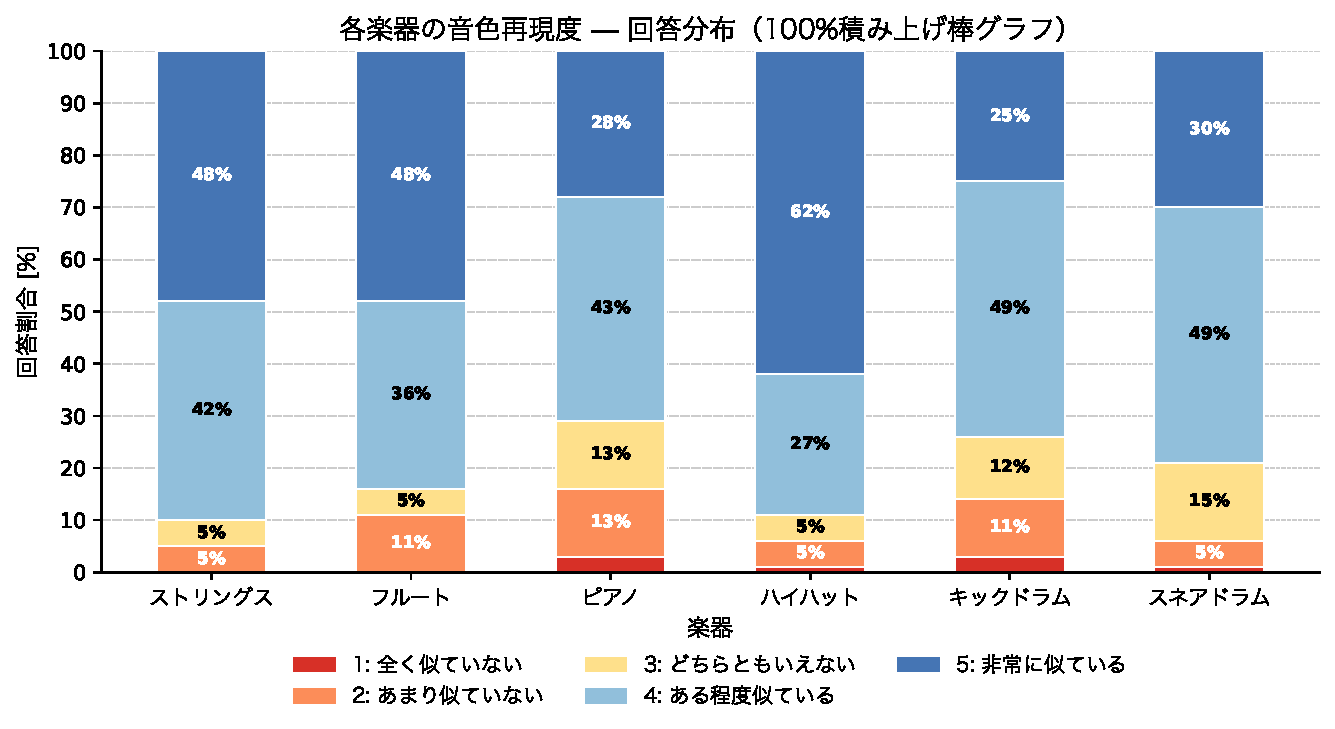
\includegraphics[width=0.92\textwidth]{figs/stacked_bar.pdf}
  \caption{各楽器の音色再現度に対する回答分布（100\%積み上げ棒グラフ）}
  \label{fig:stacked_bar}
\end{figure}

\begin{figure}[htbp]
  \centering
  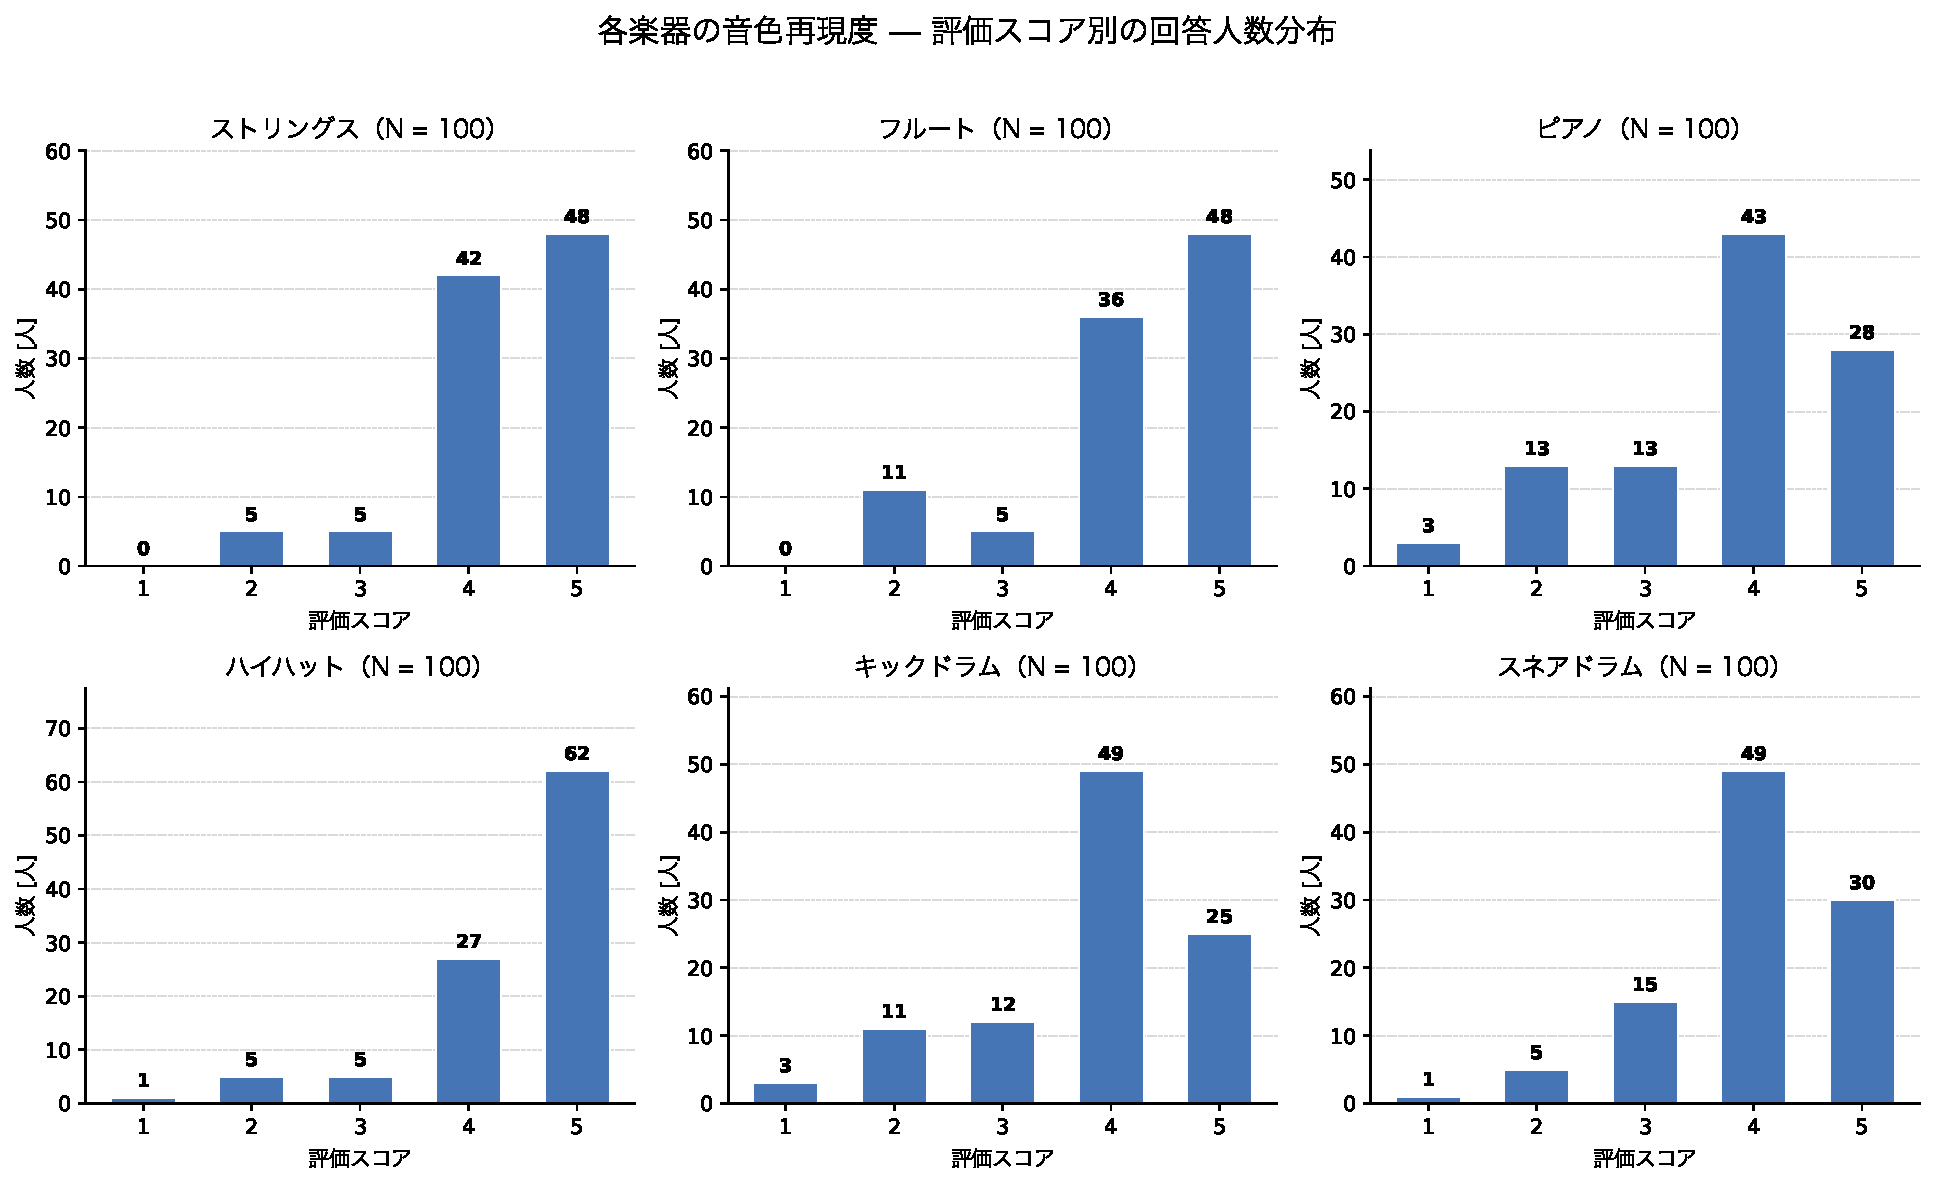
\includegraphics[width=\textwidth]{figs/score_histogram.pdf}
  \caption{各楽器の評価スコア別の回答人数分布}
  \label{fig:score_histogram}
\end{figure}

ハイハットは評価5（非常に似ている）の回答が62\%と最も高い割合を示し，評価4以上の回答が合計89\%を占めた．ストリングスおよびフルートにおいても評価4以上の割合はそれぞれ90\%，84\%であり，高い類似度が認められた．一方，キックドラムでは評価3以下の回答が26\%を占め，6楽器中で最も低い類似度の分布を示した．ピアノについても評価3以下の割合が29\%と比較的高い値を示した．

各楽器の中央値・最頻値および四分位数（$Q_1$，$Q_3$，IQR）と，MOPの目標値（中央値および最頻値がともに4.0以上）に基づく判定結果を表~\ref{tab:median_mode}に示す．また，中央値・最頻値をMOP目標値とともに視覚化した棒グラフを図~\ref{fig:mos_median_mode}に示す．

\begin{table}[htbp]
  \centering
  \caption{各楽器のMOS評価（中央値・最頻値・四分位数）とMOP判定結果（$N = 100$，MOP目標値：中央値・最頻値$\geq 4.0$）}
  \label{tab:median_mode}
  \begin{tabular}{lcccccc}
    \hline
    楽器 & 中央値 & 最頻値 & $Q_1$ & $Q_3$ & IQR & MOP判定 \\
    \hline
    ストリングス & 4 & 5 & 4 & 5 & 1 & 達成 \\
    フルート     & 4 & 5 & 4 & 5 & 1 & 達成 \\
    ピアノ       & 4 & 4 & 3 & 5 & 2 & 達成 \\
    ハイハット   & 5 & 5 & 4 & 5 & 1 & 達成 \\
    キックドラム & 4 & 4 & 3 & 4 & 1 & 達成 \\
    スネアドラム & 4 & 4 & 4 & 5 & 1 & 達成 \\
    \hline
  \end{tabular}
\end{table}

\begin{figure}[htbp]
  \centering
  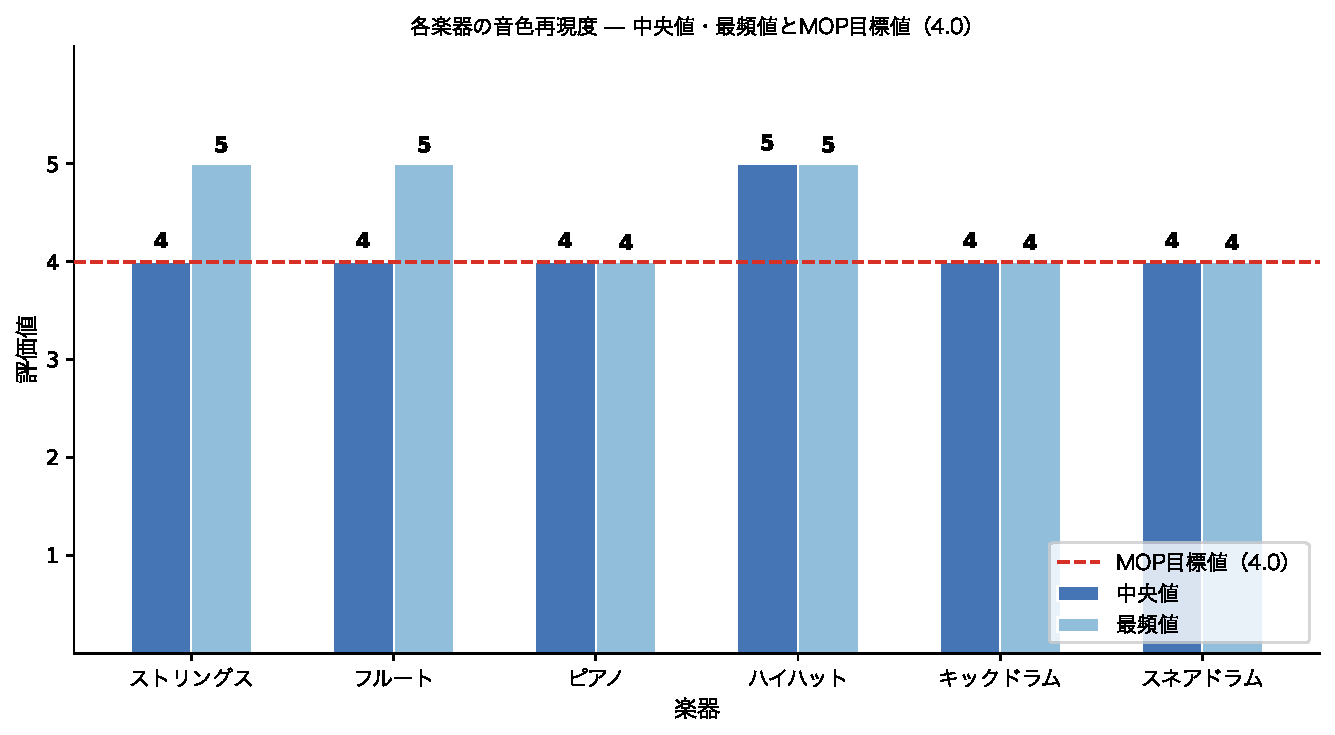
\includegraphics[width=0.92\textwidth]{figs/mos_median_mode.pdf}
  \caption{各楽器の中央値・最頻値とMOP目標値（4.0）の比較}
  \label{fig:mos_median_mode}
\end{figure}

表~\ref{tab:median_mode}に示す通り，全6楽器において中央値および最頻値はともに4.0以上であり，MOS評価に基づくMOPは全楽器で達成された．特にハイハットは中央値・最頻値がともに5であり，6楽器中で最も高い評価を得た．ストリングスおよびフルートは最頻値が5を示し，高い再現性が確認された．一方，回答分布の散らばりに着目すると，ピアノおよびキックドラムは$Q_1$が3であり，回答の4分の1以上が評価3以下に分布している．特にピアノはIQRが2と6楽器中で最も大きく，被験者間で評価が分かれたことを示している．すなわち，MOPの目標値は全楽器で達成されたものの，ピアノおよびキックドラムについては他の4楽器と比較して低評価側への分布の広がりが認められた．

% --- 以下，CSATスコアによる結果（旧版）はMOS評価への変更に伴いコメントアウト ---
% 各楽器のCSATスコア（評価4または5と回答した割合）を，非標準化（点推定のみ）および標準化（95\%Wilson信頼区間\cite{wilson1927}を用いた判定）の両方で算出した．結果を表~\ref{tab:csat_result}に，非標準化の結果を図~\ref{fig:csat_raw}に，標準化の結果を図~\ref{fig:csat_wilson}に示す．
%
% \begin{table}[htbp]
%   \centering
%   \caption{各楽器のCSATスコアとMOP判定結果（$N = 100$，MOP目標値75\%）}
%   \label{tab:csat_result}
%   \resizebox{\textwidth}{!}{%
%   \begin{tabular}{lrrrcc}
%     \hline
%     楽器 & Top2Box人数 & CSATスコア[\%] & 95\%Wilson信頼区間[\%] & MOP判定（非標準化） & MOP判定（標準化） \\
%     \hline
%     ストリングス & 90 & 90.0 & [82.6, 94.5] & 達成   & 達成   \\
%     フルート     & 84 & 84.0 & [75.6, 89.9] & 達成   & 達成   \\
%     ピアノ       & 71 & 71.0 & [61.5, 79.0] & 未達成 & 未達成 \\
%     ハイハット   & 89 & 89.0 & [81.4, 93.7] & 達成   & 達成   \\
%     キックドラム & 74 & 74.0 & [64.6, 81.6] & 未達成 & 未達成 \\
%     スネアドラム & 79 & 79.0 & [70.0, 85.8] & 達成   & 未達成 \\
%     \hline
%   \end{tabular}%
%   }
% \end{table}
%
% \begin{figure}[htbp]
%   \centering
%   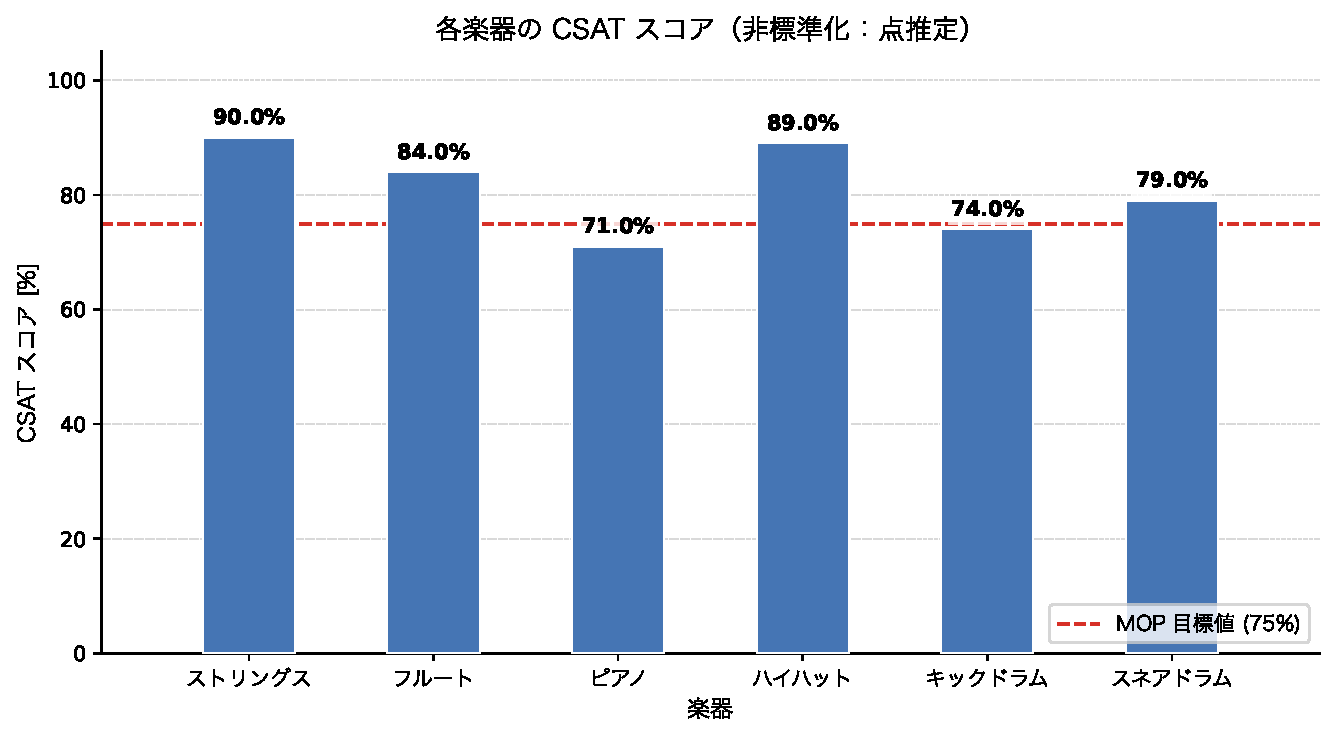
\includegraphics[width=0.92\textwidth]{figs/csat_raw.pdf}
%   \caption{各楽器のCSATスコア（非標準化：点推定）とMOP目標値（75\%）の比較}
%   \label{fig:csat_raw}
% \end{figure}
%
% \begin{figure}[htbp]
%   \centering
%   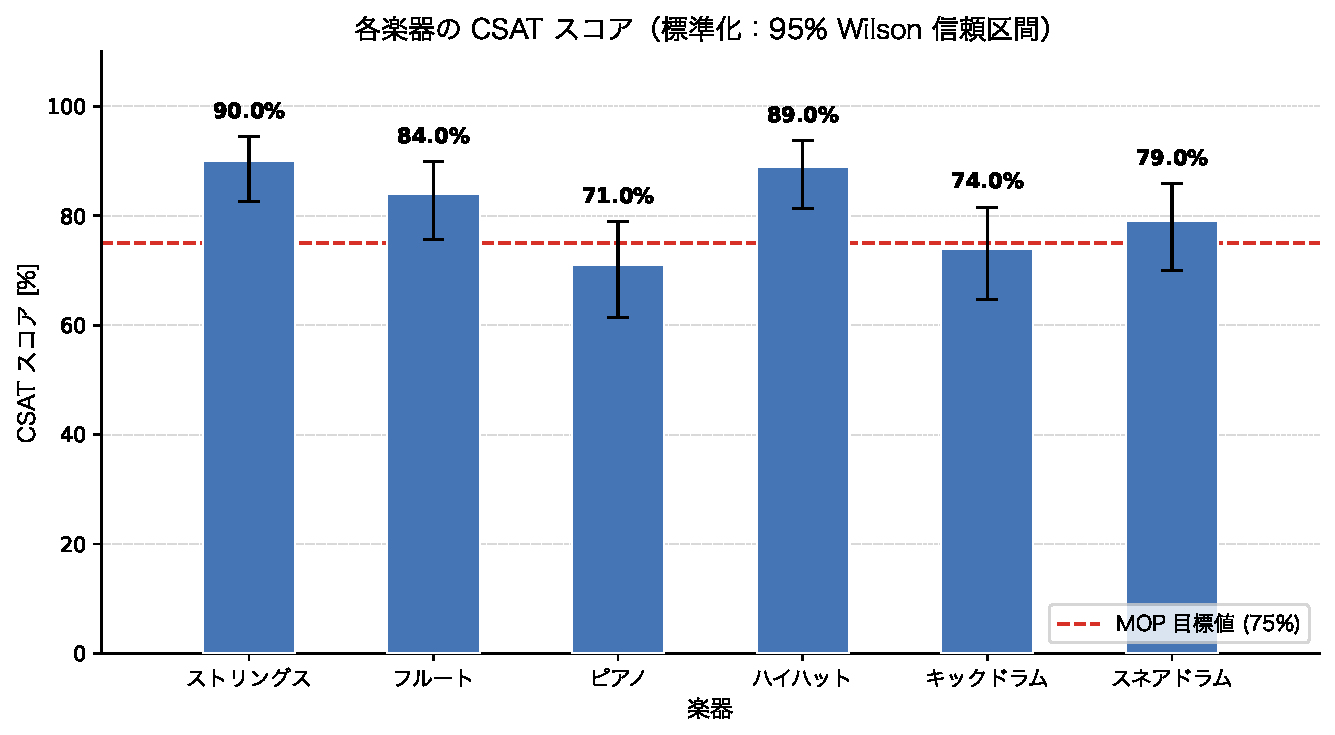
\includegraphics[width=0.92\textwidth]{figs/csat_wilson.pdf}
%   \caption{各楽器のCSATスコア（標準化：95\%Wilson信頼区間）とMOP目標値（75\%）の比較}
%   \label{fig:csat_wilson}
% \end{figure}
%
% 表~\ref{tab:csat_result}に示す通り，非標準化（点推定）で判定した場合，ストリングス，フルート，ハイハット，スネアドラムの4楽器がMOPの目標値である75\%以上を達成した．一方，ピアノおよびキックドラムは，それぞれCSATスコア71.0\%，74.0\%であり，点推定の段階でMOPを達成しなかった．
%
% 標準化（95\%Wilson信頼区間の下限による判定）で判定した場合，達成と判定された楽器はストリングス，フルート，ハイハットの3楽器にとどまった．スネアドラムは点推定では79.0\%とMOPを上回っていたものの，95\%信頼区間の下限が70.0\%であり，サンプルサイズに基づく推定の不確実性を考慮すると，MOPを安定して達成しているとは言い切れない結果となった．ピアノおよびキックドラムは，非標準化・標準化のいずれにおいてもMOPを達成しなかった．
%
% 以上より，非標準化・標準化のいずれにおいてもMOPを達成したのはストリングス，フルート，ハイハットの3楽器であった．ピアノおよびキックドラムは，非標準化・標準化のいずれにおいてもMOPを達成しなかった．スネアドラムは，非標準化では達成と判定されたが，標準化では未達成と判定された．






\FloatBarrier

\subsection{結合テスト}
\subsubsection{評価方法}
\label{sec:ketsugo_method}

結合テストでは，中継機デバイス本体のハードウェア実装と回転制御プログラム，楽器デバイスの受光部と楽曲表現プログラム，および指揮デバイスからのBPM・音量指令を行う通信部を結合した段階で評価を行う．本システムは，指揮デバイスと観覧車型の中継機・楽器デバイスを用いた空間的なフィードバックにより，利用者に高い没入感を与えることを目的として設計されている．そのため，結合テストでは，利用者がこの空間的フィードバックを違和感なく体験できているかという知覚・体験の観点から，「輪唱のタイミングに対して不快に感じる程度の遅延がないか」，「ユーザの操作が正しく反映されるか」，「エンターテイメント性があるか」の3点をMOE（Measure of Effectiveness：効果指標）として定める．これらは，本システムが技術的に動作するだけでなく，利用者の体験として意図した効果を実際に発揮しているかを確認するために設定したものである．

まず，輪唱のタイミングに対して不快に感じる程度の遅延がないかについて評価する．これは，各楽器デバイスの発音タイミングにズレが生じた際，利用者がそれを違和感なく1つの輪唱として聴取できるかを確認するものである．MOPの目標値は，ハース効果\cite{haas1951}（時間差を伴う類似した2つの音を，一定時間内であれば聴覚が1つの音として知覚する現象）の許容限界である\SI{50}{ms}未満とする．なお，\ref{sec:gakki_naibu}項で述べた同期通信（演奏開始時刻を事前に指定して伝える'O'通信の冗長送信等）は，このMOPを満たすことを目的として実装されたものであり，結合テストではこの機構が実際に機能しているかを合わせて確認する．

次に，ユーザの操作が正しく反映されるかについて評価する．評価方法としては，\ref{sec:tanka_method}項（単体テスト）で述べたボタン判定の制御テストおよびBPM・音量読み取りテストと同様に，各デバイスを結合した状態でボタン押下から中継機デバイスの動作反映までの成功率，および指揮棒の操作によるBPM・音量変更が実際に発音へ反映される成功率を計測する．MOPの目標値は，処理成功率99.0\%以上とする．この99\%（ツーナイン）という基準は，一般的なWebサービス等の開発環境において目標とされる稼働率の数値\cite{kobesoft_availability}を参考としたものであり，本プロジェクトで作成するシステムはブレッドボード上で稼働する一つのシステムであるため，テスト環境での運用に近いことから，この数値を目標として採用した．

次に，エンターテイメント性があるかについて評価する．評価方法としては，同様にアンケート調査を実施する．具体的には，「観覧車の回転と楽器が演奏をしている様子を見て，空間的な楽しさや驚きに満足したか？」，「指揮棒を振ったり，可変抵抗器を操作して，演奏のテンポなどがリアルタイムに変化する操作感に満足したか？」，および「光と音の動きが一体になったアトラクションとして，総合的な楽しさに満足したか？」という3つの質問を，1（不満）〜5（大変満足）の5段階リッカート尺度で回答してもらう．MOPの目標値は，ユーザの操作評価と同様に，CSATスコアが75\%以上\cite{acsi}とする．また，CSATスコアはアンケートという有限のサンプルから得られた比率の点推定値であり，サンプルサイズに依存した推定の不確実性を伴うため，点推定のみによる判定（非標準化）に加えて，95\%Wilson信頼区間\cite{wilson1927}の下限値による判定（標準化）を併用する．

結合テストで評価する項目とMOPの目標値を表\ref{table:ketsugo_mop}に示す．

\begin{table}[H]
    \caption{結合テストで評価する性能指標（MOP）}
    \label{table:ketsugo_mop}
    \centering
    \begin{tabular}{p{4cm}p{9cm}}
    \hline
    \textbf{評価項目} & \textbf{評価方法とMOP目標値} \\ \hline\hline
    輪唱タイミングの遅延 & 演奏開始から発音までの時間および楽器間の演奏ズレをミリ秒単位で計測．\SI{50}{ms}未満\cite{haas1951}\\ \hline
    ユーザ操作の反映度 & ボタン押下からの動作反映成功率，およびBPM・音量変更の発音反映成功率を計測．処理成功率99.0\%以上\cite{kobesoft_availability}\\ \hline
    エンターテイメント性 & 空間的な楽しさ等に関するアンケート調査（5段階リッカート尺度）．CSATスコア75\%以上\cite{acsi}\\ \hline
    \end{tabular}
\end{table}

\subsubsection{結果}
\label{sec:ketsugo_result}

まず，輪唱のタイミングに対して不快に感じる程度の遅延がないかについて評価する．同期開始条件を\SI{50}{ms}以下とした場合，一度同期が確立した後の楽器間の演奏タイミングのズレはMOPの目標値である\SI{50}{ms}未満に収まり，輪唱のタイミングに関するMOPは満たされることが確認された．しかしながら，\ref{sec:tanka_result}項（単体テスト）で示した通り，同期開始条件を\SI{50}{ms}以下と厳格に設定すると，同期の確立自体（ボタン押下から楽曲再生開始までの応答遅延）に時間を要し，全53回の試行のうち8回がTanらの示す\SI{60}{s}\cite{tan2026}の閾値を超過するという結果が得られている．したがって，輪唱タイミングのズレそのものに関するMOPは満たされる一方，そのタイミングを実現するまでの過程においては応答遅延に関するMOPを満たせない場合があることに留意する必要がある．

次に，ユーザの操作が正しく反映されるかについて評価する．\ref{sec:tanka_result}項（単体テスト）で示した通り，全160回のボタン押下試行のうち158回で中継機デバイスが正常に動作し，成功率は98.8\%であった．また，指揮デバイスを振ることによるBPM・音量の変更についても，全ての試行において意図した段階が正しく反映され，多重検知や停止状態での誤反応は確認されなかった．以上より，ボタン押下による操作反映の成功率（98.8\%）は，MOPの目標値である処理成功率99.0\%以上をわずかに下回ったものの，指揮棒操作によるBPM・音量変更の反映については誤動作なく機能しており，全体としてはユーザの操作がほぼ意図通りに反映されることが確認された．

続いて，エンターテイメント性があるかについて評価する．被験者18名に対する回答の度数分布を表~\ref{tab:entertainment_distribution}に，各質問・各評価スコアの回答人数（サンプル数$N$を含む）を示すヒストグラムを図~\ref{fig:entertainment_score_histogram}に示す．

\begin{table}[htbp]
    \centering
    \caption{エンターテイメント性アンケートに対する回答の度数分布（$N = 18$）}
    \label{tab:entertainment_distribution}
    \resizebox{\textwidth}{!}{%
    \begin{tabular}{lrrrrr}
    \hline
    質問項目 & 1 & 2 & 3 & 4 & 5 \\
             & 不満 & (未使用) & どちらともいえない & 満足 & 大変満足 \\
    \hline
    空間的な楽しさや驚き & 0 & 0 & 0 & 5 & 13 \\
    操作感               & 1 & 0 & 1 & 9 & 7  \\
    総合的な楽しさ       & 0 & 0 & 1 & 4 & 13 \\
    \hline
    \end{tabular}%
    }
\end{table}

\begin{figure}[htbp]
    \centering
    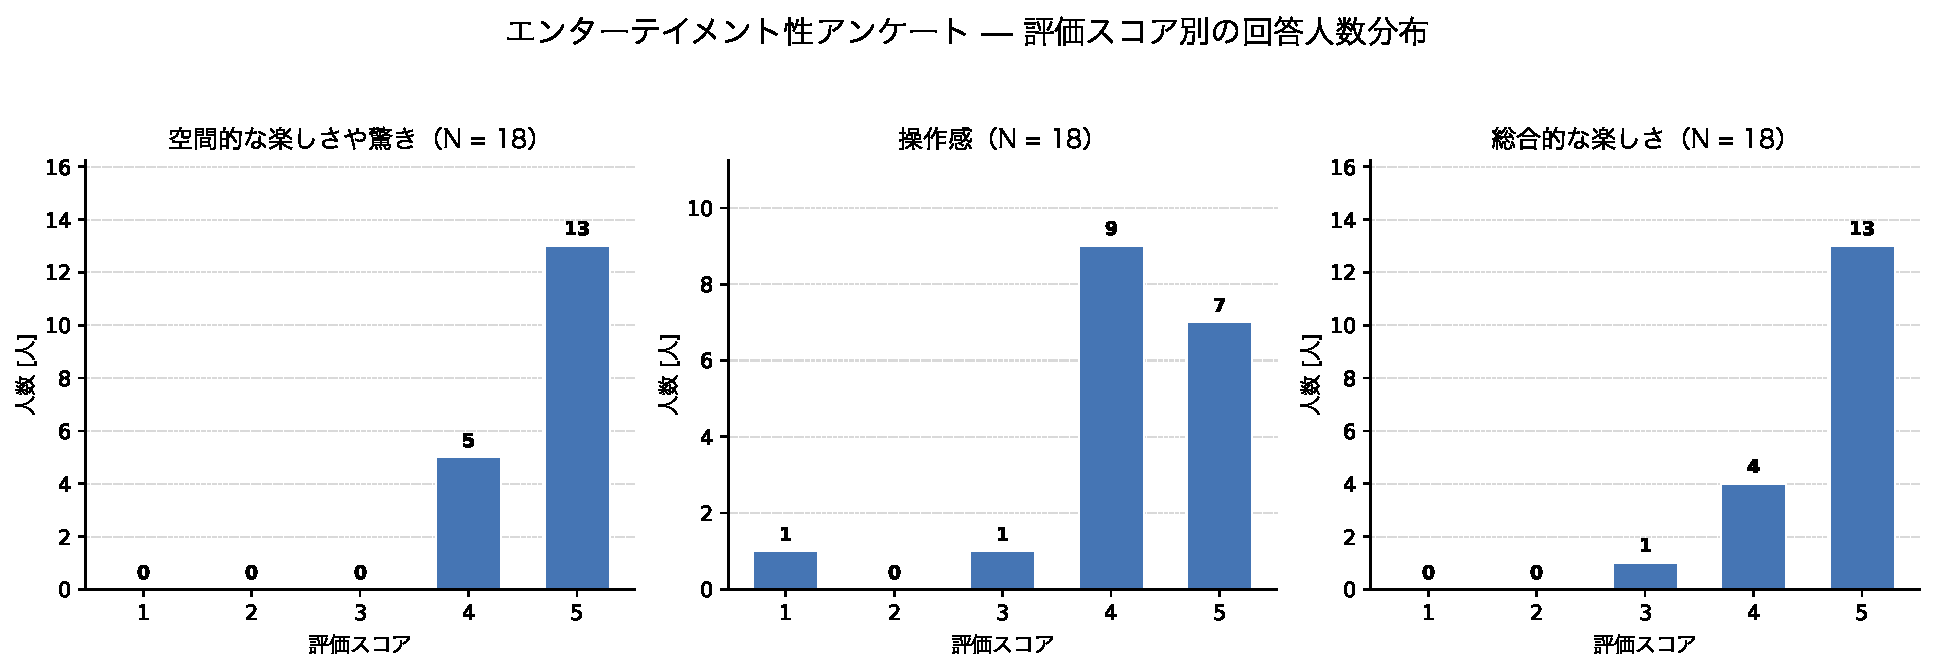
\includegraphics[width=\textwidth]{figs/entertainment_score_histogram.pdf}
    \caption{エンターテイメント性アンケートの評価スコア別の回答人数分布}
    \label{fig:entertainment_score_histogram}
\end{figure}

CSATスコアは，非標準化（点推定のみ）および標準化（95\%Wilson信頼区間\cite{wilson1927}の下限による判定）の両方で算出した．算出結果を表~\ref{tab:csat_entertainment}に，非標準化の結果を図~\ref{fig:csat_entertainment_raw}に，標準化の結果を図~\ref{fig:csat_entertainment_wilson}に示す．

\begin{table}[htbp]
    \centering
    \caption{エンターテイメント性アンケートのCSATスコアとMOP判定結果（MOP目標値75\%）}
    \label{tab:csat_entertainment}
    \resizebox{\textwidth}{!}{%
    \begin{tabular}{lrrrcc}
    \hline
    質問項目 & Top2Box人数 & CSATスコア[\%] & 95\%Wilson信頼区間[\%] & MOP判定（非標準化） & MOP判定（標準化） \\
    \hline
    空間的な楽しさや驚き & 18/18 & 100.0 & [82.4, 100.0] & 達成   & 達成   \\
    操作感               & 16/18 &  88.9 & [67.2,  96.9] & 達成   & 未達成 \\
    総合的な楽しさ       & 17/18 &  94.4 & [74.2,  99.0] & 達成   & 未達成 \\
    \hline
    \end{tabular}%
    }
\end{table}

\begin{figure}[htbp]
    \centering
    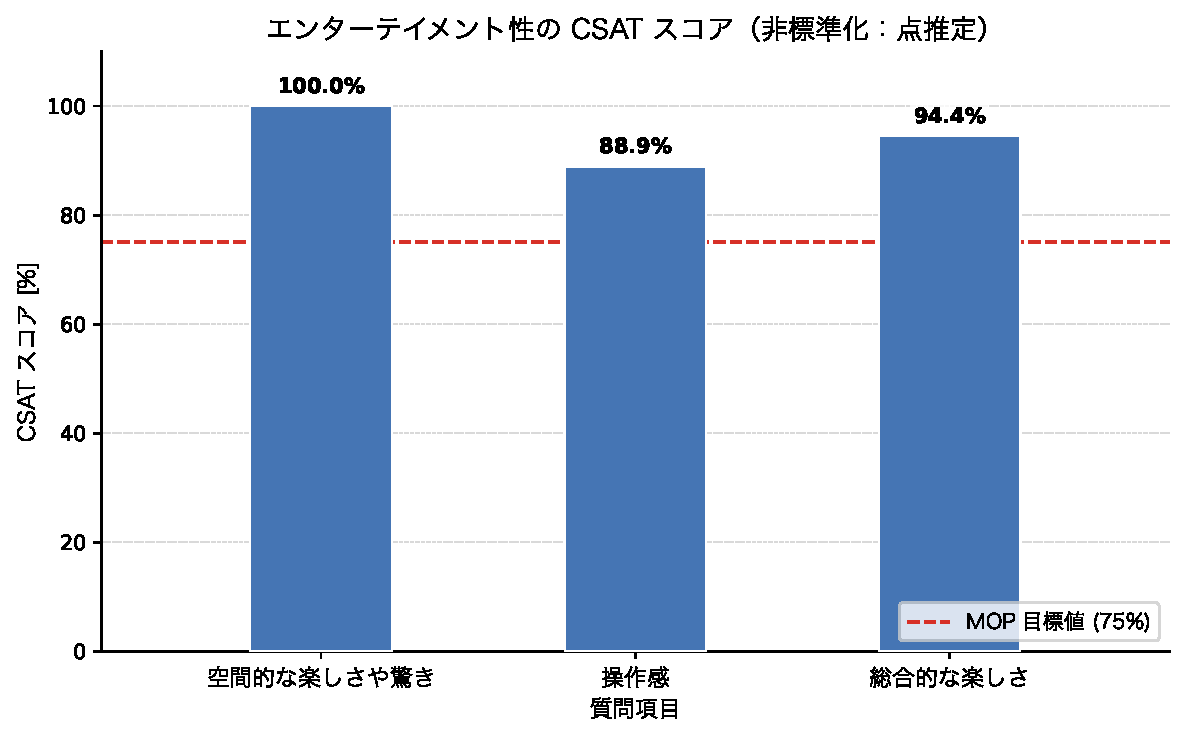
\includegraphics[width=0.85\textwidth]{figs/csat_entertainment_raw.pdf}
    \caption{エンターテイメント性のCSATスコア（非標準化：点推定）とMOP目標値（75\%）の比較}
    \label{fig:csat_entertainment_raw}
\end{figure}

\begin{figure}[htbp]
    \centering
    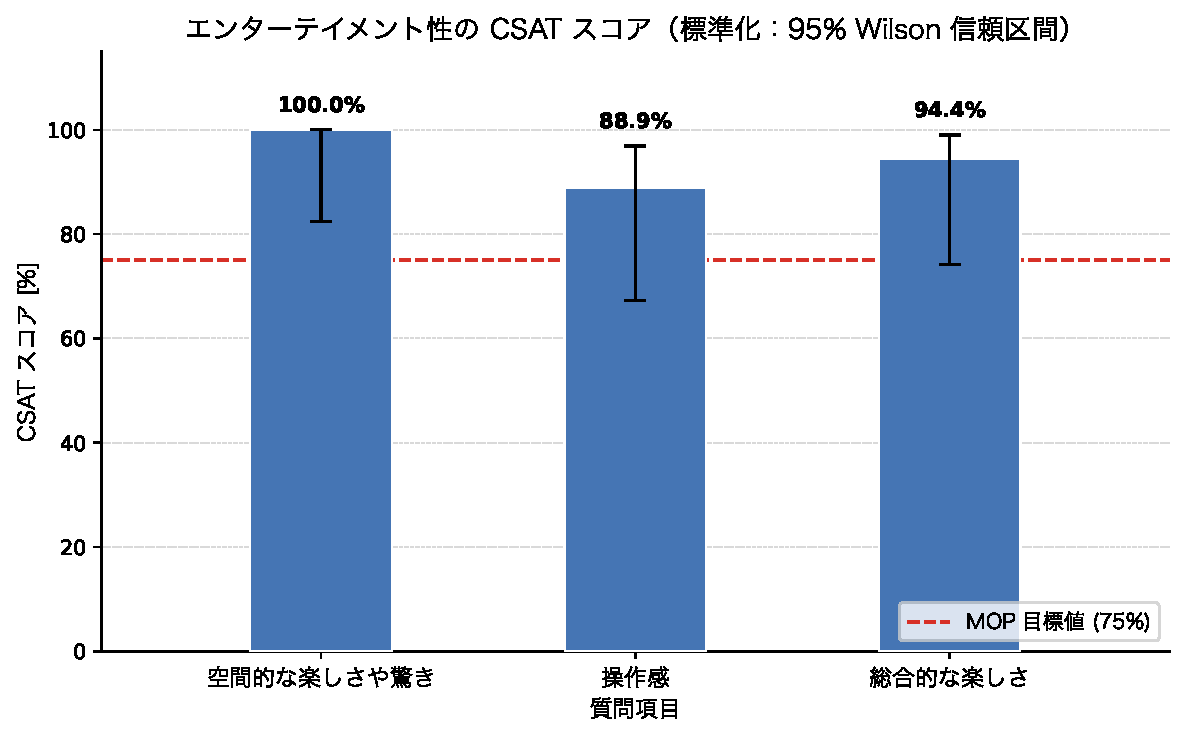
\includegraphics[width=0.85\textwidth]{figs/csat_entertainment_wilson.pdf}
    \caption{エンターテイメント性のCSATスコア（標準化：95\%Wilson信頼区間）とMOP目標値（75\%）の比較}
    \label{fig:csat_entertainment_wilson}
\end{figure}

表~\ref{tab:csat_entertainment}に示す通り，非標準化（点推定）で判定した場合，3項目すべてがMOPの目標値である75\%以上を達成した．特に「空間的な楽しさや驚き」については18名全員が4（満足）または5（大変満足）と回答し，CSATスコアは100.0\%であった．

一方，標準化（95\%Wilson信頼区間の下限による判定）で判定した場合，MOPを達成したのは「空間的な楽しさや驚き」の1項目のみであった．「操作感」および「総合的な楽しさ」は，点推定ではそれぞれ88.9\%，94.4\%であったが，95\%信頼区間の下限値はそれぞれ67.2\%，74.2\%であり，いずれも75\%の目標値を下回った．

